% To familiarize yourself with this template, the body contains
% some examples of its use.  Look them over.  Then you can
% run LaTeX on this file.  After you have LaTeXed this file then
% you can look over the result either by printing it out with
% dvips or using xdvi.
%

\documentclass[twoside]{article}
%\usepackage{soul}
\usepackage{./lecnotes_macros}


\begin{document}
%FILL IN THE RIGHT INFO.
%\lecture{**LECTURE-NUMBER**}{**DATE**}{**LECTURERS**}{**SCRIBE**}
\lecture{4}{Cryptanalysis of the full DES}{Maria Francis and M. V. Panduranga Rao}{Gautam Singh}{27 January 2025}
%\footnotetext{These notes are partially based on those of Nigel Mansell.}

%All figures are to be placed in a separate folder named ``images''

% **** YOUR NOTES GO HERE:

The iterative characteristic by itself is not enough to break 16-round DES due
to its low probability. However, it was enough for DES reduced to 15 rounds. To
retain this probability, we use a new round 1. This new round 1 will generate
plaintexts with XOR \(\brak{\psi,0}\) which can then be fed into the
characteristic. This gives rise to a modified 2R-attack which is fast enough to
break DES. We describe the various stages of the attack below.

\section{Data Collection Phase}

We require to generate data whose XORed inputs into the iterative characteristic
are \(\brak{\psi, 0}\). Suppose \(P\) is a 64-bit plaintext and let \(v_i\) be a
32-bit constant with the first 12 bits equal to the possible outputs of S1, S2,
S3 after the first round and 0 elsewhere for \(0 \le i < 2^{12}\). Define for
\(0 \le i < 2^{12}\)

\begin{align}
    P_i = P \oplus \brak{v_i, 0} \quad & \bar{P_i} = \brak{P \oplus \brak{v_i, 0}} \oplus \brak{0, \psi} \label{eq:pi-def} \\
    T_i = \textrm{DES}\brak{P_i, K} \quad & \bar{T_i} = \textrm{DES}\brak{\bar{P_i}, K}. \label{eq:ti-def}
\end{align}

Then, \(P_i \oplus \bar{P_j} = \brak{v_k, \psi}\). Out of the \(2^{24}\)
possibilities of \(\brak{i, j}\), each \(v_k\) occurs exactly \(2^{12}\) times.
Now, an XOR of \(\psi\) is fed into the first round, but we do not know which
\(v_k\) is to be chosen initially to cancel the output of the \(F\) function and
give us the desired \(\brak{\psi, 0}\) input to the second round. 

However, trying all \(2^{24}\) possibilities is slow. To find the right \(v_k\),
we exploit the cross-product structure of \(P_i\) and \(\bar{P_j}\). Notice that
a right pair will have zero outputs at S4, \dots, S8 of the last round. Thus, we
can feed in the plaintexts \(P_i\) and \(\bar{P_j}\) to get outputs \(T_i\) and
\(\bar{T_j}\). These \(2^{13}\) outputs can then be hashed by these 20
positions. A right pair will survive with probability \(2^{-20}\). Thus, out of
the \(2^{24}\) pairs, we will get only \(2^{4} = 16\) pairs.

We can further filter these pairs by testing against S boxes in rounds 1, 15 and
16. The input XOR values of S1, S2 and S3 in the first and the fifteenth rounds
are fixed for right pairs. For the other boxes, we use the fact that about 80 \%
of the XOR pairs are possible. This reduces the number of surviving pairs to a
fraction \(\brak{\frac{14}{16} \cdot \frac{13}{16} \cdot \frac{15}{16}}^2 \cdot
0.8^8 = 0.0745\) of the original. Now, we are left with \(16 \cdot 0.0745 =
1.19\) pairs per structure. Although right pairs are filtered, some wrong pairs
may not have been filtered.

\section{Data Analysis Phase}

In previous attacks, data analysis entailed counting on certain subkey bits and
then trying the most popular key values. This is memory intensive. In contrast,
this attack uses negligible space by trying each suggested key value. A key
value is suggested when it can create the output XOR of the last round and the
expected output XOR of the first round using the particular plaintext and
ciphertext pairs.

In the first and fifteenth rounds, the XOR inputs to S4, \dots, S8 are all zero.
The DES key scheduling algorithm ensures that all 28 key bits of the left
register enters S1, S2 and S3 in the last two rounds and 24 key bits of the
right register are used in the last round. Thus, \(28 + 24 = 52\) bits enter the
S boxes of the last two rounds. Considering there are \(2^{32} \cdot 0.8^8\)
possible outputs for the last round, there are only \(X =
\frac{2^{-32}}{0.8^8}\) fraction of keys left. Considering S1, S2 and S3 in each
of the first and fifteenth rounds gives the factor \(Y =
\frac{2^{-12}}{\frac{14}{16}\cdot\frac{13}{16}\cdot\frac{15}{16}}\) for each
round. Putting it all together, each pair suggests \(2^{52}XY^2 = 0.84\) values
of these 52 bits. Thus, each structure suggests \(1.19 \cdot 0.84 \cdot 2^4 =
16\) choices for the whole key. To check whether a key is the right one, we can
``peel'' up the two additional rounds for each ciphertext pair and verify
against against the characteristic, totaling to \(16 \cdot 2 \cdot \frac{2}{16}
= 4\) DES operations. The signal-to-noise ratio of this counting scheme is \(S/N
= \frac{2^{52} \cdot 2^{-47.2}}{\frac{1.19}{2^{12}} \cdot 0.84} = 2^{16.8}\).

We now describe the actual data analysis and extraction of the suggested keys.
For the left register, we enumerate the 64 possibilities of \(S4_{Kh}\), leaving
on average 4 possibilities. From \autoref{fig:des-k1-k16}, notice that three
bits of \(S4_{Kh}\) are shared with \(S3_{Ka}\). Enumerating the other three
bits reduces the average number of possibilities to two. Two bits of \(S1_{Kh}\)
are shared with \(S3_{Ka}\). By completing the missing bits of \(S1_{Kh}\) and
then the two missing bits of \(S2_{Ka}\), we can reduce the number of
possibilities to about half on average. Completing the other 13 remaining bits
of the left register in a similar way reduces the average number of suggested
values of the left register to one. Similar counting methods are used on the
right register to deduce 24 out of the 28 bits.

\begin{figure}[!ht]
    \centering
    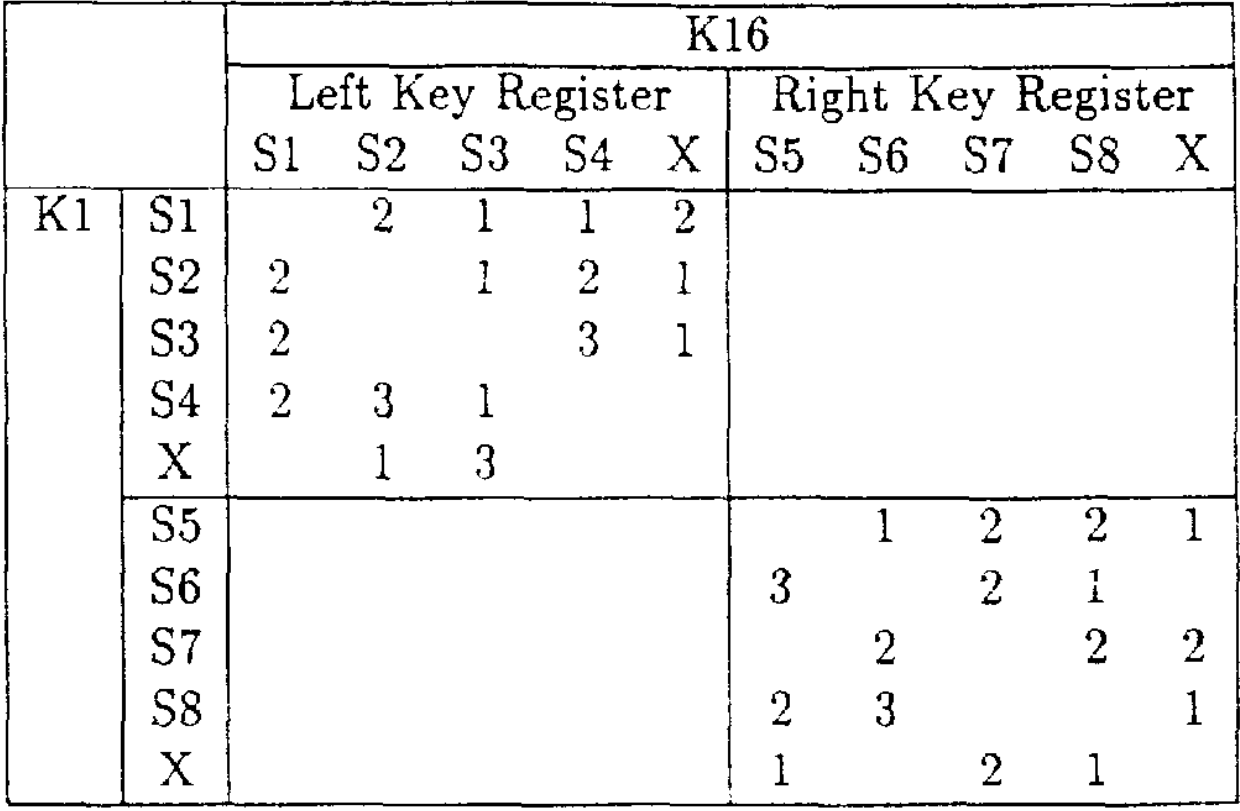
\includegraphics[width=0.5\textwidth]{images/des-k1-k16.png}
    \caption{Number of common key bits in K1 and K16.}
    \label{fig:des-k1-k16}
\end{figure}

\section{Summary and Complexity}

In summary, the following steps are performed to attack the entire 16 round DES.

\begin{enumerate}
    \item Each structure contains a right pair with probability \(2^{-35.2}\).
    The data collection phase uses \(2^{35}\) structures, from which about
    \(2^{35} \cdot 1.19 = 2^{35.25}\) pairs survive.
    \item The probability that one of them is a right pair is about 58 \%.
    \item Analysis of the right pair leads to the correct key with high
    probability.
\end{enumerate}

The time complexity of this attack is about \(2^{35} \cdot 4 = 2^{37}\)
equivalent DES operations.

A further reduction can be used by creating metastructures using the iterative
characteristic with \(\psi = \texttt{1B 60 00 00}_x\). This metastructure would
contain \(2^{14}\) plaintexts.

We can parallelize the processing of each of these structures on up to
\(2^{33}\) processors with small local memories, one for each structure. Another
advantage of this attack is that it can be done even when keys are changed
frequently during data collection. The attack can be carried out incrementally
with the number of available pairs, with success probabilities increasing with
each new pair.

\section{General Form of the Attack}

The general form of this attack is stated in \autoref{thm:gen-attack} without
proof.

\begin{theorem}
\label{thm:gen-attack}    
Given a characteristic with probability \(p\) and signal-to-noise ratio \(S/N\)
for an iterated cryptosystem with \(k\) key bits, we can apply an attack which
encrypts \(\frac{2}{p}\) chosen plaintexts in the data collection phase and
whose complexity is \(\frac{2^k}{S/N}\) encryptions during the data analysis
phase.
\end{theorem}

Appropriately chosen metastructures can reduce the number of plaintexts to
\(\frac{1}{p}\). Further, the effective time complexity can be reduced by a
factor of \(f \le 1\) if a wrong key can be discarded by carrying out a fraction
\(f\) of the rounds.
\end{document}
